As hard radiation cannot be stopped by a moderate lead thickness so cosmic vetos are employed, which consists of at least two complementary detectors in coincidence that reject events simoultaneously detected in both. 

As shown in Figure \ref{fig:VetoAndPrototype}, the two complementary detectors are placed one above and the other below the TIRTIUM detector. The distance between both detectors, $34.2~\cm$ for our latest prototype developed, is set by the TRITIUM prototype to be placed between both.

\begin{figure}[h]
\centering
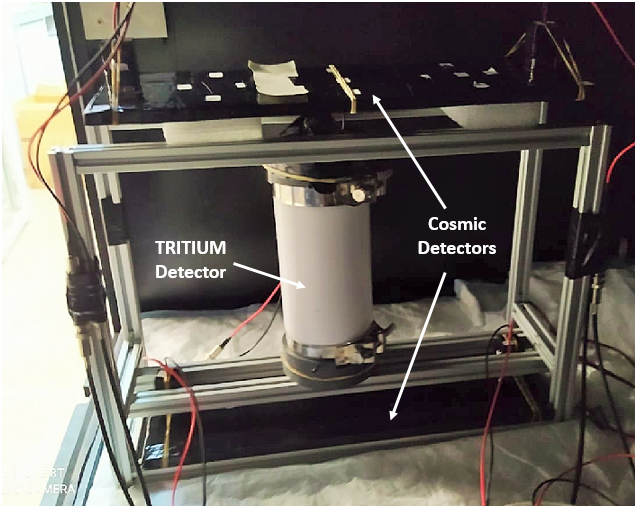
\includegraphics[scale=0.45]{3DesignPrinciples/34BackgroundRejectionSystem/Vetos_y_prototipo.png}
\caption{Cosmic veto and Tritium-IFIC 2 prototype in an aluminum mechanical structure developed by IFIC's mechanical engineering department.\label{fig:VetoAndPrototype}}
\end{figure}

A hard cosmic event simultaneous through both cosmic detectors is schematically shown in figure \ref{subfig:RealHardCosmicEvent}. Each cosmic detector has two photosensors so the electronic configuration given in Figure \ref{subfig:ElectronicConfiguraiton4PMT} is used in each active veto to make time coincidences. The TRITIUM detector is read out in anti-coincidence with the cosmic veto to rejected the hard cosmic events from the tritium measurement. Random coincidence from two different hard cosmic events, one in each detector, shown in Figure \ref{subfig:FakeHardCosmicEvent} are negligible. The expected hard cosmic rate at sea level for muons, main contributor, is $70~\meter^{-2}\second^{-1}\steradian^{-1}$ \cite{PDG, HardCosmicMuonRate}, that is $7\times 10^{-3}~\cm^{-2}\second^{-1}\steradian^{-1}$, shown in the cosmic rate plot of Figure \ref{fig:HardCoscmicRate}. As time coincidences are triggered by logical gates of about $10~\nano\second$, the probability of recording two different hard cosmic events in temporal coincidence is less than $10^{-9}$ which is not worth considering.

\begin{figure}
\centering
    \begin{subfigure}[b]{0.45\textwidth}
    \centering
    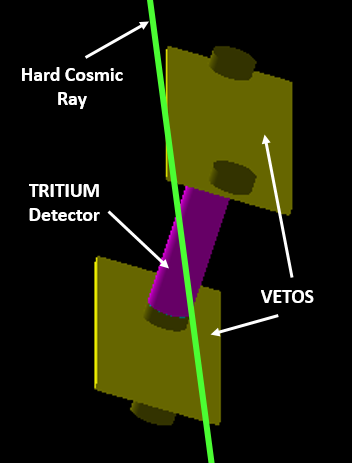
\includegraphics[width=\textwidth]{3DesignPrinciples/34BackgroundRejectionSystem/Real_Event.png}  
    \caption{Real hard cosmic event.\label{subfig:RealHardCosmicEvent}}
    \end{subfigure}
    \hfill
    \begin{subfigure}[b]{0.45\textwidth}
    \centering
    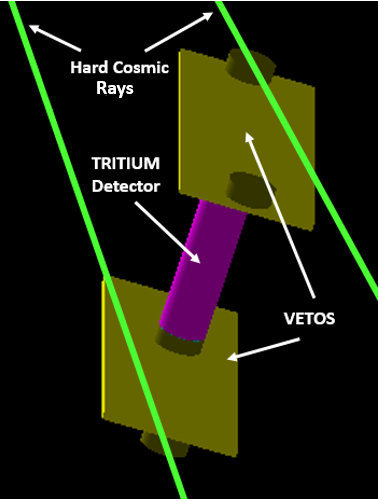
\includegraphics[width=\textwidth]{3DesignPrinciples/34BackgroundRejectionSystem/Fake_Event.png}  
    \caption{Fake hard cosmic event.\label{subfig:FakeHardCosmicEvent}}
    \end{subfigure}
   \caption{Hard cosmic events detected with the cosmic veto of TRITIUM: a) Affecting to the tritium measurement, b) Does not affecting to the tritium measurement.}
 \label{fig:HardCosmicEventsSimulation}
\end{figure}

\begin{figure}[h]
\centering
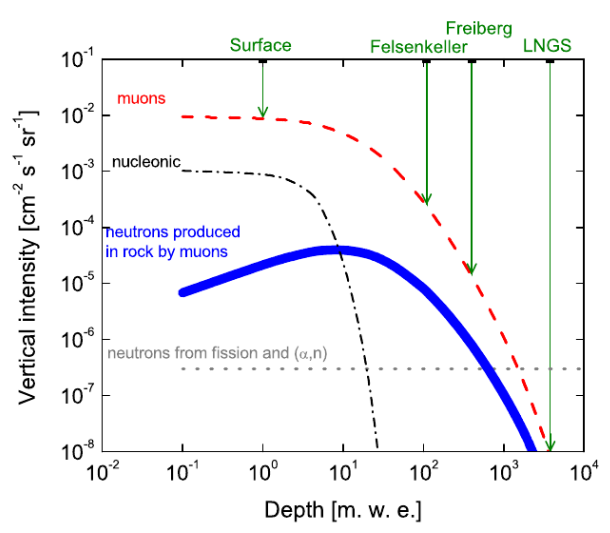
\includegraphics[scale=0.6]{3DesignPrinciples/34BackgroundRejectionSystem/HardCosmicRate.png}
\caption{Hard cosmic muon rate \cite{HardCosmicMuonRatePlot}.\label{fig:HardCoscmicRate}}
\end{figure}

The vetos are made of a plastic scintillator block from Epic-Crystal \cite{ScintillatorVeto}. Its properties are given in Table \ref{tab:ParametersScintillatorVeto} and its energy emission spectrum is displayed in Figure \ref{fig:EmissionEnergySpectrumVeto}.

\begin{table}[]
%%\centering
\begin{center}
\begin{tabular}{|c|c|c|}
%\hline
%Material & Refractive index \\
\hline \hline 
Base material & Polystyrene \\ \hline
Growth method & Polymeric \\ \hline
Density ($\gram/\cm^3$)& 1.05 \\ \hline
Refractive index & 1.58 \\ \hline
Soften temperature ($\degree$) & 75-80 \\ \hline
Light output (Anthracene) & 50-60\% \\ \hline
H/C raito & 1.1 \\ \hline
Emission peak (nm) & 415 (Blue) \\ \hline
Decay Time, (ns) & 2.4 \\ \hline
Hygroscopic & No \\ \hline
\end{tabular}
\caption{Properties of plastic scintillators from Epic-Crystals~\cite{ScintillatorVeto}.}
\label{tab:ParametersScintillatorVeto}
\end{center}
\end{table}

\begin{figure}[]
\centering
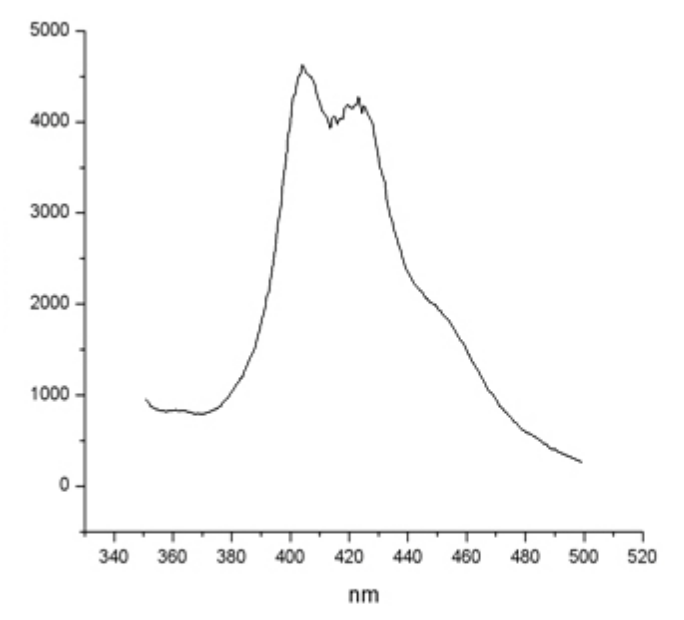
\includegraphics[scale=0.35]{3DesignPrinciples/34BackgroundRejectionSystem/EmissionEnergySpectrumVetos.png}
\caption{Emission energy spectrum of the plastic scintillation used for the cosmic vetos\label{fig:EmissionEnergySpectrumVeto}~\cite{ScintillatorVeto}.}
\end{figure}

The energy spectrum has a peak very close to that of the scintillating fibers used, so the same photosensors are used to read out them. The dimensions of the scintillator block are $45 \cdot{} 17 \dot{} 1~\cm^3$ and they are wrapped by three different layers, teflon, aluminum and black tape, exhibited in Figure \ref{fig:LayersVeto}. These layers prevent external photons from reaching the scintillator plastic and avoid photons generated by the scintillator plastic from escaping before reaching the photosensor. Two $2.5\times 2.5 ~\cm^2$ windows are made on the wrapping to allow reading by the photosensors.


\begin{figure}
\centering
    \begin{subfigure}[b]{0.23\textwidth}
    \centering
    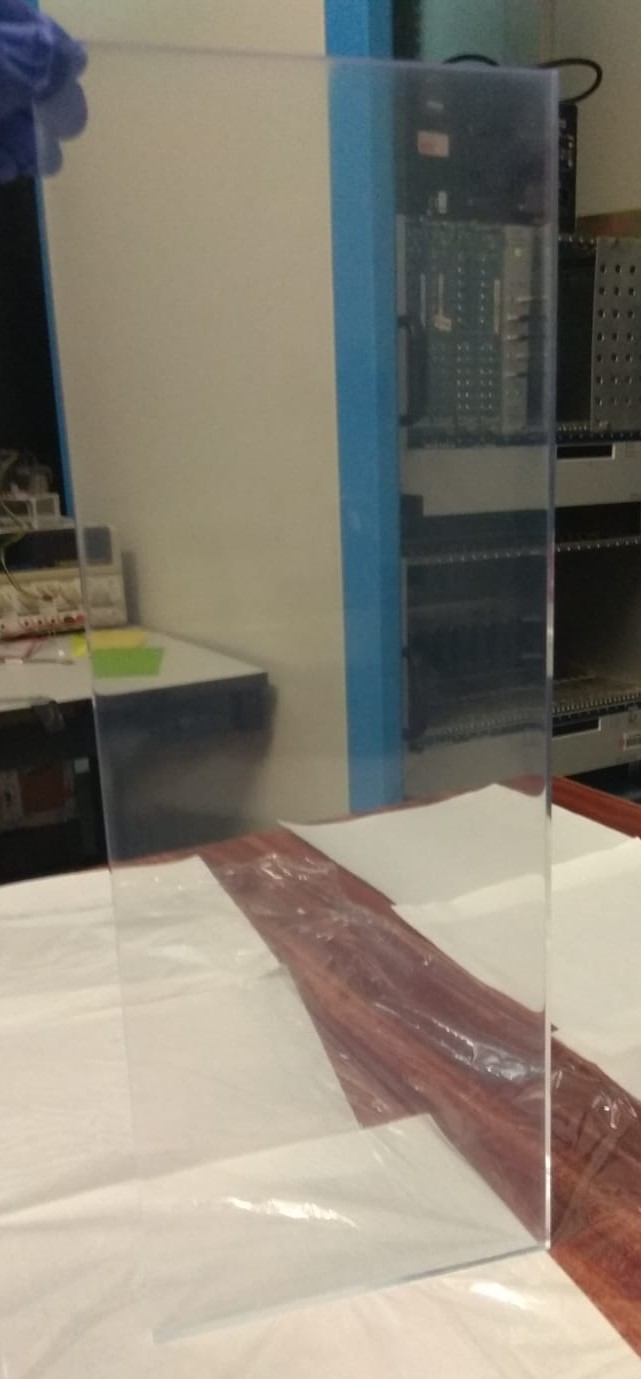
\includegraphics[width=\textwidth]{3DesignPrinciples/34BackgroundRejectionSystem/NoCoating.jpeg}  
    \caption{Scintillator without coating.\label{subfig:PlasticScintillatorNoCoating}}
    \end{subfigure}
    \hfill
    \begin{subfigure}[b]{0.23\textwidth}
    \centering
    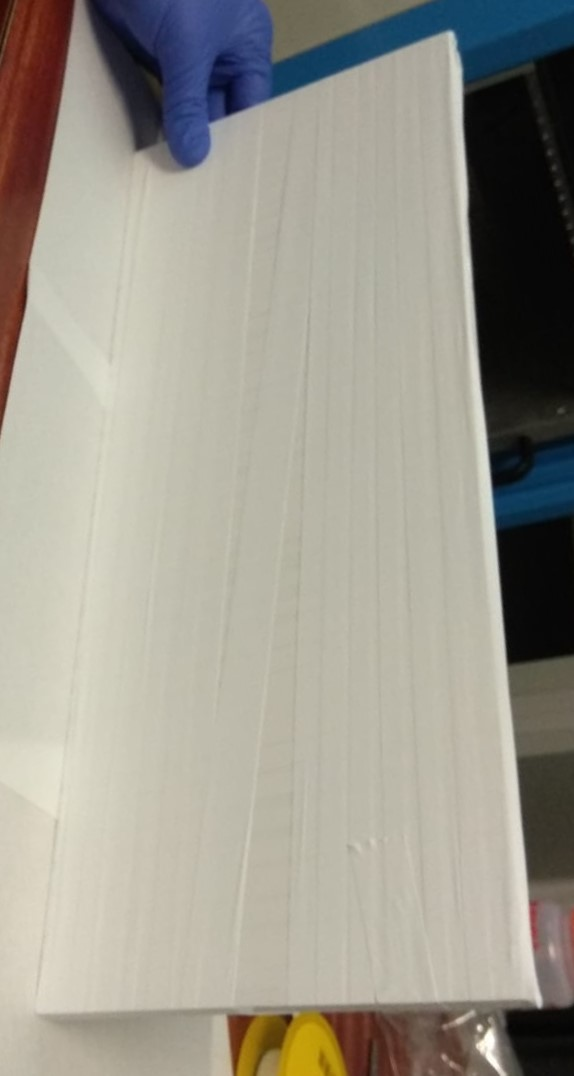
\includegraphics[width=\textwidth]{3DesignPrinciples/34BackgroundRejectionSystem/TeflonCoating.jpeg}  
    \caption{Teflon coating.\label{subfig:PlasticScintillatorTeflon}}
    \end{subfigure}
    \hfill
    \begin{subfigure}[b]{0.23\textwidth}
    \centering
    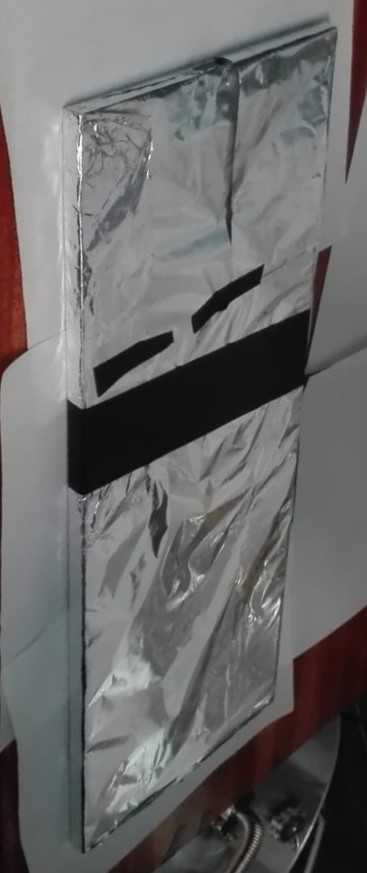
\includegraphics[width=\textwidth]{3DesignPrinciples/34BackgroundRejectionSystem/AluminiumCoating.jpeg}  
    \caption{Aluminium coating.\label{subfig:PlasticScintillatorAluminium}}
    \end{subfigure}
    \hfill
    \begin{subfigure}[b]{0.23\textwidth}
    \centering
    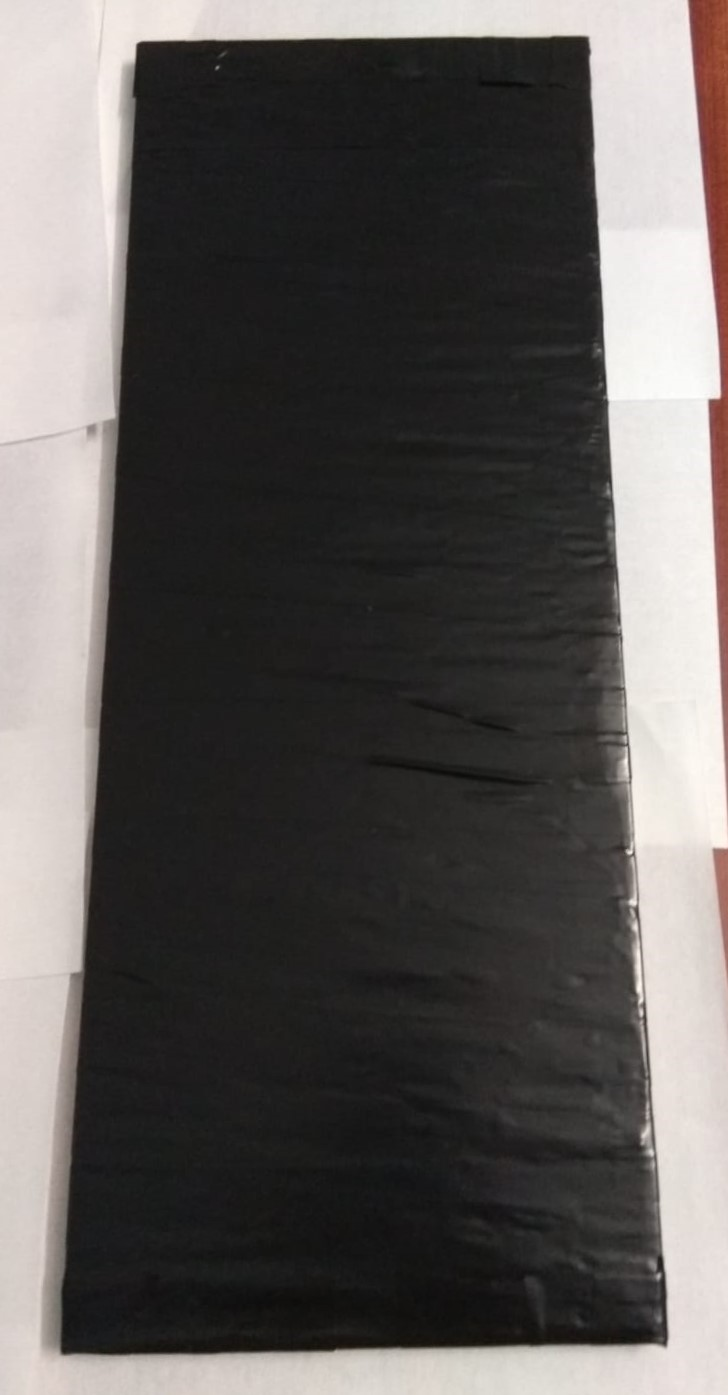
\includegraphics[width=\textwidth]{3DesignPrinciples/34BackgroundRejectionSystem/BlackTapeCoating.jpeg}  
    \caption{Black tape coating.\label{subfig:PlasticScintillatorBlackTape}}
    \end{subfigure}
 \caption{Different layers used to cover of the cosmic veto.}
 \label{fig:LayersVeto}
\end{figure}

As previously mentioned, the expected hard cosmic rate at sea level is $7 \times 10^{-3}~\cm^{-2}\second^{-1}\steradian^{-1}$. Taking into account that the solid angle of our detectors is $\omega=0.5434$, calculated by integrating the solid angle of one scintillator on the other, and the area of the veto is $765~\cm^2$, the expected hard cosmic rate on our cosmic vetos should be $2,909~$event$/\second$. This is an important result which is used in section \ref{sec:TritiumActiveVeto} to determine the efficiency of the cosmic veto.